% ============================================================================
% Մանկավարժական լուծումներ - Դիսկրետ մաթեմատիկա, Գործնական 4 (Ֆունկցիաներ).
% Խնդիրներ 2, 4, 5, 6, 10, 12, 19, 22, 24, 25.
% Հայերեն տարբերակ, XeLaTeX (fontspec + Sylfaen). Կազմել՝ xelatex-ով երկու անգամ։
% Տերմինաբանությունը՝ glossary_discrete_focused.md / glossary_Apr.csv-ի համաձայն։
% ============================================================================
\documentclass[11pt,a4paper]{article}

% ---- Տառատեսակ (XeLaTeX) ----
\usepackage{fontspec}
\setmainfont{Sylfaen}

% Հայերենը plain XeLaTeX-ում տողադարձման կանոններ չունի, ուստի երկար տողերը չեն
% կարող կոտրվել և դուրս կգան լուսանցքից։ Թող TeX-ը ձգի բառամիջյան բացատները։
\tolerance=2000
\emergencystretch=3.5em

% ---- Մաթեմատիկա ----
\usepackage{amsmath,amssymb,amsthm}
\usepackage{mathtools}

% ---- Դասավորություն ----
\usepackage[margin=2.3cm]{geometry}
\usepackage{enumitem}
\usepackage{booktabs}
\usepackage{array}

% ---- Գրաֆիկա ----
\usepackage{xcolor}
\usepackage[most]{tcolorbox}
\usepackage{tikz}
\usetikzlibrary{arrows.meta,positioning,calc,fit,backgrounds,shapes.misc,shapes.geometric,decorations.pathreplacing}
\usepackage{pgfplots}
\pgfplotsset{compat=1.18}
\usepackage{hyperref}
\hypersetup{colorlinks=true,linkcolor=blue!55!black,urlcolor=blue!55!black}

% ---- Գունապնակ (Հայաստանի դրոշի գույները) ----
\definecolor{armRed}{HTML}{D90012}
\definecolor{armBlue}{HTML}{0033A0}
\definecolor{armOrange}{HTML}{F2A800}
\definecolor{ink}{HTML}{22303C}

\setlength{\parindent}{0pt}
\setlength{\parskip}{5pt}

% ---- Մաթեմատիկական կրճատումներ ----
\newcommand{\Z}{\mathbb{Z}}
\newcommand{\R}{\mathbb{R}}
\newcommand{\N}{\mathbb{N}}
\newcommand{\Q}{\mathbb{Q}}
\newcommand{\dom}{\operatorname{dom}}
\DeclareMathOperator{\Ker}{Ker}
\DeclareMathOperator{\im}{Im}

% ---- Վանդակներ ----
\newtcolorbox{problembox}[1][]{enhanced, breakable, sharp corners=south,
  colback=armOrange!10, colframe=armOrange!75!black, boxrule=0.8pt, arc=2mm,
  fonttitle=\bfseries\color{white}, coltitle=white,
  attach boxed title to top left={xshift=4mm,yshift=-2.4mm},
  boxed title style={colback=armOrange!85!black, arc=1mm},
  title={Խնդիր #1}}

\newtcolorbox{ideabox}{enhanced, breakable,
  colback=armBlue!6, colframe=armBlue!70!black, boxrule=0.8pt, arc=2mm,
  fonttitle=\bfseries\color{white}, coltitle=white,
  attach boxed title to top left={xshift=4mm,yshift=-2.4mm},
  boxed title style={colback=armBlue!75!black, arc=1mm},
  title={Գաղափարը}}

\newtcolorbox{methodbox}{enhanced, breakable,
  colback=gray!8, colframe=gray!55!black, boxrule=0.7pt, arc=2mm,
  fonttitle=\bfseries, title={$\bigstar$\ Հիշարժան մեթոդ}}

\newtcolorbox{answerbox}{enhanced, sharp corners=south,
  colback=green!8, colframe=green!50!black, boxrule=1pt, arc=2mm, left=4mm,right=4mm}
\newcommand{\answer}[1]{\begin{answerbox}\centering\textbf{Պատասխան՝}\quad #1\end{answerbox}}

% ---- Վերնագիր ----
\title{\vspace{-1.2cm}\textbf{Դիսկրետ մաթեմատիկա - Գործնական 4}\\[2pt]
\large Ֆունկցիաներ՝ մանրամասն լուծումներ\\[2pt]
\normalsize\itshape դատողությունները՝ քայլ առ քայլ բացված}
\author{}
\date{}

\begin{document}
\maketitle
\vspace{-1.0cm}

\begin{center}\small\itshape Ընդգրկում է Գործնական 4-ի հանձնարարված խնդիրները՝ 2, 4, 5, 6, 10, 12, 19, 22, 24, 25։\end{center}

\section*{Նախապատրաստում}

\emph{Ֆունկցիան} $f:A\to B$ կանոն է, որը \textbf{յուրաքանչյուր} մուտքին $x\in A$ վերագրում է ճիշտ
մեկ ելք $f(x)\in B$։ $A$ բազմությունը \textbf{որոշման տիրույթն} է (որտեղ կանոնին թույլատրվում է
գործել), իսկ իրականում արտադրված արժեքների բազմությունը՝ $\{f(x):x\in A\}$, \textbf{արժեքների
տիրույթն} է (կամ պատկերը)։ Այս թերթիկը չորս տեսակի հարց է տալիս։ (1) \textbf{Որոշման և արժեքների
տիրույթը կարդալ} բանաձևից (խնդիր 2)՝ որտեղ է բանաձևը օրինական, և ինչ արժեքներ են դուրս գալիս։
(2) \textbf{Համադրել} երկու ֆունկցիա և գտնել \textbf{հակադարձներ} (խնդիրներ 4, 5)։ (3) Ֆունկցիան
\textbf{դասակարգել} որպես ինյեկտիվ, սյուրյեկտիվ կամ բիյեկտիվ (խնդիրներ 6, 12)։ (4) \textbf{Դատել
բազմությունների պատկերների և նախապատկերների մասին} (խնդիրներ 10, 19, 22, 24, 25), որտեղ ողջ խաղն
այն է, թե արդյոք $f$-ը ինյեկտիվ է։

\begin{tcolorbox}[colback=armRed!6,colframe=armRed!70!black,boxrule=0.8pt,arc=2mm,
  title={\bfseries Մի պայմանավորվածություն, որ պետք է ֆիքսել մյուս ամեն ինչից առաջ՝ համադրումը ձախից աջ է},
  fonttitle=\bfseries\color{white},coltitle=white]
Այս դասընթացում ֆունկցիաների կետային արտադրյալը կարդացվում է \textbf{ձախից աջ}՝ $f\cdot g$ նշանակում է
«նախ արա $f$, ապա $g$», ուստի
\[
  (f\cdot g)(x) \;=\; g\bigl(f(x)\bigr)։
\]
Սա \emph{հակառակն} է $\circ$ սիմվոլի, որ թերևս տեսել ես, որտեղ $g\circ f$ նշանակում է
$g(f(x))$։ Ստորև ամենուր օգտագործում ենք դասընթացի պայմանավորվածությունը՝ խնդիր 4-ն այնտեղ է, որ
սա կծում է, ուստի հետևիր կարգին։ Մտածիր այն որպես խողովակաշար՝ մուտքը նախ հոսում է \emph{ձախ} արկղով։
\end{tcolorbox}

\begin{center}
\begin{tikzpicture}[font=\small,>=Stealth,
  box/.style={draw,rounded corners=2pt,minimum width=1.5cm,minimum height=8mm,fill=armBlue!12}]
\node (x) at (0,0) {$x$};
\node[box] (f) at (2.2,0) {$f$};
\node[box] (g) at (5.0,0) {$g$};
\node (out) at (8.4,0) {$g(f(x))=(f\cdot g)(x)$};
\draw[->,thick] (x) -- (f);
\draw[->,thick] (f) -- node[above]{$f(x)$} (g);
\draw[->,thick] (g) -- (out);
\node[armRed] at (3.6,-0.9) {\itshape ձախ արկղը նախ է գործում};
\end{tikzpicture}
\end{center}

% ============================================================================
\section*{Խնդիր 2 - Որոշման և արժեքների տիրույթը բանաձևից}

\begin{problembox}[2]
Դիցուք $f\subseteq\R\times\R$։ Գտիր որոշման և արժեքների տիրույթը յուրաքանչյուր բանաձևի համար՝
\[
\text{(ա) } x^2+3,\quad
\text{(բ) } \sqrt{x-2},\quad
\text{(գ) } \tfrac{1}{\sqrt{x-2}},\quad
\text{(դ) } |x|,\quad
\text{(ե) } \tfrac{1}{x^2+2},\quad
\text{(զ) } \tfrac{1}{x^2-2}.
\]
\end{problembox}

\begin{ideabox}
Երկու առանձին հարց, որ կարդացվում են գրաֆիկից։ \textbf{Որոշման տիրույթը} «որտեղ է բանաձևը
օրինական» հարցն է՝ խուսափիր միայն երկու վտանգից՝ \emph{քառակուսի արմատի տակ բացասական արժեքից} և
\emph{հայտարարում զրոյից}՝ մնացած ամեն ինչ թույլատրելի է, ուստի որոշման տիրույթը ողջ $\R$-ն է՝
հանած այդ արգելված կետերը։ \textbf{Արժեքների տիրույթը} «ինչ բարձրությունների է հասնում գրաֆիկը»
հարցն է՝ կառուցիր այն ներսից դեպի դուրս։ $\tfrac{1}{x^2-2}$-ի նման բանաձևի համար նախ տես, թե ինչ
կարող է լինել $u=x^2-2$-ը, ապա տես, թե $\tfrac1u$-ն ինչ է անում այդ բազմությանը։ Հակադարձ արժեքը
շրջում է միջակայքի կարգը և $0$-ին մոտ արժեքներն ուղարկում $\pm\infty$, ինչը ճիշտ պատճառն է, որ (զ)-ի
արժեքների տիրույթը բաժանվում է երկու կտորի։
\end{ideabox}

\textbf{Քայլ 1 - Որոշման տիրույթներ (գտիր արգելված կետերը)։}
(ա),(դ),(ե) չունեն ոչ արմատ, ոչ հայտարար, և $x^2+2\ge2>0$, ուստի օրինական են ամենուր՝
որոշման տիրույթը $\R$ է։ (բ) $\sqrt{x-2}$-ի համար պետք է $x-2\ge0$, այսինքն $x\ge2$։ (գ)
$\tfrac1{\sqrt{x-2}}$-ի համար արմատը պետք է լինի օրինական \emph{և} ոչ զրոյական, ուստի $x-2>0$,
այսինքն $x>2$։ (զ) $\tfrac1{x^2-2}$-ի համար պետք է $x^2-2\ne0$, այսինքն $x\ne\pm\sqrt2$։

\textbf{Քայլ 2 - Արժեքների տիրույթներ (աշխատիր ներսից դեպի դուրս)։}
(ա) $x^2\ge0\Rightarrow x^2+3\ge3$, $\ge3$ ամեն արժեքին հասնում ենք, արժեքների տիրույթը $[3,\infty)$ է։
(բ) $\sqrt{\,\cdot\,}\ge0$ և անսահման աճում է, արժեքների տիրույթը $[0,\infty)$ է։
(գ) $\tfrac1{\sqrt{x-2}}>0$՝ երբ $x\to2^+$, այն պայթում է, երբ $x\to\infty$, ձգտում է $0$-ի (առանց
երբևէ հասնելու դրան), արժեքների տիրույթը $(0,\infty)$ է։
(դ) $|x|\ge0$, արժեքների տիրույթը $[0,\infty)$ է։
(ե) $x^2+2\in[2,\infty)$, ուստի $\tfrac1{x^2+2}\in(0,\tfrac12]$՝ առավելագույնը՝ $\tfrac12$, $x=0$-ում է,
և արժեքները փոքրանում են դեպի $0$, երբ $|x|\to\infty$։ Արժեքների տիրույթը՝
$\bigl(0,\tfrac12\bigr]$։
(զ) Դիցուք $u=x^2-2$, ուստի $u\in[-2,\infty)\setminus\{0\}$։ $u\in[-2,0)$-ի վրա հակադարձ արժեքը տալիս է
$\tfrac1u\in(-\infty,-\tfrac12]$ ($-\tfrac12$ արժեքը գալիս է $u=-2$-ից, այսինքն $x=0$-ից)՝ իսկ
$u\in(0,\infty)$-ի վրա այն տալիս է $\tfrac1u\in(0,\infty)$։ Արժեքների տիրույթը՝
$\bigl(-\infty,-\tfrac12\bigr]\cup(0,\infty)$։

\textbf{Քայլ 3 - Միշտ ստուգիր եզրային արժեքները։}
(ե) $x=0$-ում՝ $\tfrac1{0+2}=\tfrac12$։ \checkmark\ (զ) $x=0$-ում՝ $\tfrac1{0-2}=-\tfrac12$, բացասական
ճյուղի գագաթը։ \checkmark\ Թվային ընտրանքը խիտ ցանցի վրա հաստատում է վերևի յուրաքանչյուր մինիմում/մաքսիմում։

\answer{%
(ա) $\dom=\R$, արժ. տիրույթ $[3,\infty)$;\quad
(բ) $\dom=[2,\infty)$, արժ. տիրույթ $[0,\infty)$;\quad
(գ) $\dom=(2,\infty)$, արժ. տիրույթ $(0,\infty)$;\\[2pt]
(դ) $\dom=\R$, արժ. տիրույթ $[0,\infty)$;\quad
(ե) $\dom=\R$, արժ. տիրույթ $\bigl(0,\tfrac12\bigr]$;\quad
(զ) $\dom=\R\setminus\{\pm\sqrt2\}$, արժ. տիրույթ $\bigl(-\infty,-\tfrac12\bigr]\cup(0,\infty)$.}

\medskip
\textbf{Որոշման և արժեքների տիրույթը նկարից կարդալը։} Երկու ամենապարզ դեպքերը՝ (բ) և (զ)։ (բ)-ի համար
որոշման տիրույթը $x$ առանցքի վրա փակագիծն է ($x\ge2$), իսկ արժեքների տիրույթը $y$ առանցքի վրա
փակագիծն է ($y\ge0$)։ (զ)-ի համար կորն ունի ուղղաձիգ ասիմպտոտներ $x=\pm\sqrt2$-ում և $y$ առանցքը
բաժանում է հենց արժեքների տիրույթի երկու կտորի։

\begin{center}
\begin{tikzpicture}
\begin{axis}[
  name=plotb, width=7.2cm, height=5.4cm,
  axis lines=middle, xlabel={$x$}, ylabel={$y$},
  xmin=-1.2, xmax=8, ymin=-0.8, ymax=3,
  xtick={2}, ytick={0}, xticklabels={$2$},
  title={(բ) $f(x)=\sqrt{x-2}$}, title style={font=\small},
  every axis x label/.style={at={(ticklabel* cs:1.0)},anchor=west},
  every axis y label/.style={at={(ticklabel* cs:1.0)},anchor=south}]
\addplot[domain=2:8, samples=120, very thick, armBlue]{sqrt(x-2)};
\addplot[only marks, mark=*, mark size=1.4pt, armBlue] coordinates {(2,0)};
% domain bracket on x-axis
\draw[armRed, very thick] (axis cs:2,-0.45) -- (axis cs:7.8,-0.45);
\node[armRed,font=\scriptsize,anchor=west] at (axis cs:3.3,-0.62) {որոշ. տիրույթ $[2,\infty)$};
% range bracket on y-axis
\draw[armOrange!90!black, very thick] (axis cs:-0.55,0) -- (axis cs:-0.55,2.8);
\node[armOrange!75!black,font=\scriptsize,rotate=90,anchor=south] at (axis cs:-0.85,1.2) {արժ. տիրույթ $[0,\infty)$};
\end{axis}

\begin{axis}[
  name=plotf, at={($(plotb.east)+(2.0cm,0)$)}, anchor=west,
  width=7.2cm, height=5.4cm,
  axis lines=middle, xlabel={$x$}, ylabel={$y$},
  xmin=-3.2, xmax=3.2, ymin=-3, ymax=3,
  xtick={-1.414,1.414}, xticklabels={$-\sqrt2$,$\sqrt2$},
  ytick={-0.5}, yticklabels={$-\tfrac12$},
  title={(զ) $f(x)=\dfrac{1}{x^2-2}$}, title style={font=\small},
  every axis x label/.style={at={(ticklabel* cs:1.0)},anchor=west},
  every axis y label/.style={at={(ticklabel* cs:1.0)},anchor=south}]
% positive branches (|x|>sqrt2)
\addplot[domain=1.46:3.2, samples=120, very thick, armBlue]{1/(x^2-2)};
\addplot[domain=-3.2:-1.46, samples=120, very thick, armBlue]{1/(x^2-2)};
% negative branch (|x|<sqrt2)
\addplot[domain=-1.37:1.37, samples=160, very thick, armBlue]{1/(x^2-2)};
\addplot[only marks, mark=*, mark size=1.3pt, armBlue] coordinates {(0,-0.5)};
\draw[dashed, gray] (axis cs:-1.414,-3) -- (axis cs:-1.414,3);
\draw[dashed, gray] (axis cs: 1.414,-3) -- (axis cs: 1.414,3);
% range pieces on y-axis
\draw[armOrange!90!black, very thick] (axis cs:-3.0,-3) -- (axis cs:-3.0,-0.5);
\draw[armRed, very thick] (axis cs:-3.0,0.02) -- (axis cs:-3.0,3);
\node[font=\scriptsize,anchor=west] at (axis cs:0.2,2.4) {$(0,\infty)$};
\node[font=\scriptsize,anchor=west] at (axis cs:0.2,-2.5) {$(-\infty,-\tfrac12]$};
\end{axis}
\end{tikzpicture}
\end{center}

\begin{methodbox}
\textbf{Փոխանցելի տեխնիկա՝} որոշման տիրույթ $=$ «բոլոր $x$-երը, բացի այնտեղ, որտեղ արմատը դառնում է
բացասական կամ հայտարարը՝ զրո»։ Արժեքների տիրույթ $=$ կառուցիր արժեքների բազմությունը \emph{ներսից դեպի
դուրս}՝ հետևիր, թե ինչ կարող է լինել ներքին արտահայտությունը ($x^2$, $x-2$, $x^2-2$), ապա կիրառիր
արտաքին գործողությունը ($+3$, $\sqrt{\;}$, հակադարձ արժեք)։ Հակադարձ արժեքը խորամանկն է՝ այն ուղարկում է
$(0,M]$-ը $[\tfrac1M,\infty)$, իսկ $0$-ն շրջապատող բազմությունը՝ երկու առանձին կտորի։
\end{methodbox}

% ============================================================================
\section*{Խնդիր 4 - Համադրույթներ $f\cdot g$ և $g\cdot f$}

\begin{problembox}[4]
Դիցուք $f,g:\R\to\R$։ Գտիր $f\cdot g$-ն և $g\cdot f$-ը (դասընթացի պայմանավորվածությունը՝
$(f\cdot g)(x)=g(f(x))$, նախ կիրառիր $f$)՝
\[
\text{(ա) } f(x)=x^2+1,\ g(x)=x+3;\qquad
\text{(բ) } f(x)=\sqrt{x^2+2},\ g(x)=x^2+3;
\]
\[
\text{(գ) } f(x)=\tfrac1x,\ g(x)=2x+3.
\]
\end{problembox}

\begin{ideabox}
Համադրումը պարզապես մեկ մեքենայի ելքը հաջորդ մեքենայի մեջ դնելն է։ Միակ բանը, որ պետք է ճիշտ անել,
\emph{ո՞ր մեքենան է առաջինն աշխատում}-ն է։ Դասընթացի ձախից-աջ կանոնով $f\cdot g$-ն նախ աշխատեցնում է
$f$-ը՝ վերցրու $x$, հաշվիր $f(x)$, ապա այն կերակրիր $g$-ին՝ տալով $g(f(x))$։ Ուստի $f\cdot g$
կառուցելու համար գրիր $g(\square)$ և յուրաքանչյուր $\square$ փոխարինիր $f(x)$-ի ողջ բանաձևով։ Կարգը
կարևոր է՝ ընդհանուր դեպքում $f\cdot g\ne g\cdot f$, և (ա) մասը դա ցույց է տալիս բարձրաձայն։
\end{ideabox}

\textbf{Քայլ 1 - Ֆիքսիր բաղադրատոմսը։} $(f\cdot g)(x)=g(f(x))$ ($f$-ը տեղադրիր $g$-ի մեջ)՝
$(g\cdot f)(x)=f(g(x))$ ($g$-ն տեղադրիր $f$-ի մեջ)։

\textbf{Քայլ 2 - (ա) մաս։} $f(x)=x^2+1$, $g(x)=x+3$։
\[
(f\cdot g)(x)=g(f(x))=\underbrace{(x^2+1)}_{f(x)}+3=x^2+4,\qquad
(g\cdot f)(x)=f(g(x))=\underbrace{(x+3)}_{g(x)}{}^2+1=x^2+6x+10.
\]
Երկուսը տարբեր են ($x^2+4\ne x^2+6x+10$)՝ այս խնդրի գլխավոր դասը։

\textbf{Քայլ 3 - (բ) մաս։} $f(x)=\sqrt{x^2+2}$, $g(x)=x^2+3$։
\[
(f\cdot g)(x)=g(f(x))=\bigl(\sqrt{x^2+2}\bigr)^2+3=(x^2+2)+3=x^2+5,
\]
\[
(g\cdot f)(x)=f(g(x))=\sqrt{(x^2+3)^2+2}.
\]
$f\cdot g$-ում քառակուսին և քառակուսի արմատը մաքուր կերպով չեղարկվում են, քանի որ $x^2+2\ge0$։

\textbf{Քայլ 4 - (գ) մաս։} $f(x)=\tfrac1x$, $g(x)=2x+3$։
\[
(f\cdot g)(x)=g(f(x))=2\cdot\tfrac1x+3=\tfrac2x+3,\qquad
(g\cdot f)(x)=f(g(x))=\tfrac{1}{2x+3}.
\]

\textbf{Քայլ 5 - Միշտ ստուգիր ընտրանքի կետում։} (ա) $x=1$-ում՝ $f(1)=2$, $g(2)=5$, և
$1^2+4=5$։ \checkmark\ $g\cdot f$-ի համար՝ $g(1)=4$, $f(4)=17$, և $1+6+10=17$։ \checkmark\ Երեք
մասերն էլ ու երկու կարգերն էլ թվային կերպով հաստատվեցին բազմաթիվ կետերում։

\answer{%
(ա) $f\cdot g=x^2+4$,\ \ $g\cdot f=x^2+6x+10$;\quad
(բ) $f\cdot g=x^2+5$,\ \ $g\cdot f=\sqrt{(x^2+3)^2+2}$;\quad
(գ) $f\cdot g=\tfrac2x+3$,\ \ $g\cdot f=\tfrac1{2x+3}$.}

\medskip
\textbf{Սլաքների շղթան, որ կարգն անվրեպ է դարձնում։} (ա)-ի համար $x=1$ ընտրանքի կետում երկու
համադրույթները հետևում են տարբեր ուղիների։ Վերին շարքը $f\cdot g$-ն է (դասընթացի կարգը, նախ $f$)՝ ստորին
շարքը $g\cdot f$-ն է։

\begin{center}
\begin{tikzpicture}[font=\small,>=Stealth, node distance=14mm,
  val/.style={draw,circle,inner sep=1.6pt,fill=white},
  op/.style={midway,above,font=\scriptsize}]
% f.g : x -> f -> g
\node (a0) at (0,1.4) {$x=1$};
\node[val] (a1) at (3.2,1.4) {$f(1)=2$};
\node[val] (a2) at (7.4,1.4) {$g(2)=5$};
\node[anchor=west] at (9.2,1.4) {$=(f\cdot g)(1)$};
\draw[->,thick,armBlue] (a0) -- node[op]{կիրառիր $f$} (a1);
\draw[->,thick,armBlue] (a1) -- node[op]{կիրառիր $g$} (a2);
\node[armBlue,font=\scriptsize,anchor=east] at (-0.2,1.4) {$f\cdot g$:};
% g.f : x -> g -> f
\node (b0) at (0,0) {$x=1$};
\node[val] (b1) at (3.2,0) {$g(1)=4$};
\node[val] (b2) at (7.4,0) {$f(4)=17$};
\node[anchor=west] at (9.2,0) {$=(g\cdot f)(1)$};
\draw[->,thick,armRed] (b0) -- node[op]{կիրառիր $g$} (b1);
\draw[->,thick,armRed] (b1) -- node[op]{կիրառիր $f$} (b2);
\node[armRed,font=\scriptsize,anchor=east] at (-0.2,0) {$g\cdot f$:};
\end{tikzpicture}
\end{center}
Նույն մեկնարկը $x=1$, տարբեր ավարտներ ($5$ ընդդեմ $17$)՝ համադրումը կոմուտատիվ չէ, և
ձախից-աջ կանոնն ասում է, թե որ արկղն է առաջինը գործում։

\begin{methodbox}
\textbf{Փոխանցելի տեխնիկա՝} $f\cdot g$ կառուցելու համար (դասընթացի կարգ) գրիր \emph{երկրորդ}
ֆունկցիան $g(\square)$ և $\square$-ի փոխարեն տեղադրիր ողջ \emph{առաջին} բանաձևը։ Միշտ խելամտության
ստուգում արա մեկ թվում՝ բառացիորեն քայլելով խողովակաշարով։ Եթե քո երկու համադրույթները հավասար են
դուրս գալիս ֆունկցիաների ընդհանուր զույգի համար, գրեթե հաստատ կարգը խառնել ես։
\end{methodbox}

% ============================================================================
\section*{Խնդիր 5 - Հակադարձ ֆունկցիաներ}

\begin{problembox}[5]
Գտիր հակադարձ ֆունկցիան յուրաքանչյուրի համար՝
\[
\text{(ա) } f(x)=\frac{x+4}{2},\qquad
\text{(բ) } f(x)=x^3,\qquad
\text{(գ) } f(x)=\frac{x-2}{x+3}.
\]
\end{problembox}

\begin{ideabox}
Հակադարձը $f^{-1}$ չեղարկում է $f$-ը՝ եթե $f$-ն ուղարկում է $x$-ը $y$-ի, ապա $f^{-1}$-ն ուղարկում է
$y$-ը հետ $x$-ի։ Բանաձև գտնելու համար պարզապես \emph{լուծիր $y=f(x)$-ը $x$-ի նկատմամբ}։ Ինչ էլ որ
ստանաս, $x=(\text{արտահայտություն }y\text{-ով})$, դա $f^{-1}(y)$-ն է՝ ի վերջո վերանվանիր $y$-ը
$x$-ի, եթե ուզում ես։ Երկրաչափորեն հակադարձը \textbf{գրաֆիկի հայելային պատկերն է $y=x$ ուղղի
նկատմամբ}, որովհետև մուտքի և ելքի դերերը փոխանակելը փոխանակում է երկու առանցքները։
\end{ideabox}

\textbf{Քայլ 1 - (ա) մաս։} Լուծիր $y=\tfrac{x+4}{2}$-ը՝ բազմապատկիր $2$-ով, $2y=x+4$, ուստի $x=2y-4$։
Հետևաբար $f^{-1}(x)=2x-4$։

\textbf{Քայլ 2 - (բ) մաս։} Լուծիր $y=x^3$-ը՝ վերցրու (իրական) խորանարդ արմատը, $x=\sqrt[3]{y}$։ Հետևաբար
$f^{-1}(x)=\sqrt[3]{x}$։ (Խորանարդ արմատը որոշված է բոլոր իրականների համար, ներառյալ բացասականները,
ուստի սա իսկական հակադարձ է ողջ $\R$-ի վրա՝ ինչը հենց աշխատում է, քանի որ $x^3:\R\to\R$-ը բիյեկցիա է,
ինչպես հաստատում է Խնդիր 6(գ)-ն)։

\textbf{Քայլ 3 - (գ) մաս։} Լուծիր $y=\tfrac{x-2}{x+3}$-ը։ Մաքրիր հայտարարը՝
$y(x+3)=x-2\Rightarrow yx+3y=x-2\Rightarrow x(y-1)=-2-3y$, ուստի
\[
x=\frac{-2-3y}{y-1}=\frac{3y+2}{1-y}.
\]
Հետևաբար $f^{-1}(x)=\dfrac{3x+2}{1-x}$ (որոշված է $x\ne1$-ի համար՝ $1$ արժեքը հենց այն բարձրությունն է,
որին գրաֆիկը երբեք չի հասնում՝ իր հորիզոնական ասիմպտոտը)։

\textbf{Քայլ 4 - Միշտ ստուգիր՝ $f^{-1}$-ն իսկապես չեղարկում է $f$-ը։}
(ա) $f^{-1}(f(x))=2\cdot\tfrac{x+4}{2}-4=(x+4)-4=x$։ \checkmark\
(գ) վերցրու $x=0$՝ $f(0)=\tfrac{-2}{3}$, ապա $f^{-1}\!\bigl(-\tfrac23\bigr)
=\tfrac{3(-2/3)+2}{1-(-2/3)}=\tfrac{0}{5/3}=0$։ \checkmark\ Երկու ուղղություններն էլ ստուգված են
թվային կերպով։

\answer{(ա) $f^{-1}(x)=2x-4$;\quad (բ) $f^{-1}(x)=\sqrt[3]{x}$;\quad
(գ) $f^{-1}(x)=\dfrac{3x+2}{1-x}$ \ ($x\ne1$-ի համար).}

\medskip
\textbf{Հակադարձը $y=x$-ի նկատմամբ արտացոլում է։} Ահա (ա) մասը՝ $f(x)=\tfrac{x+4}{2}$ ուղիղը
և իր հակադարձը $f^{-1}(x)=2x-4$-ը հայելային պատկերներ են կետագիծ անկյունագծում։ Ընտրիր ցանկացած
կետ մի գրաֆիկի վրա, փոխանակիր նրա կոորդինատները, և կհայտնվես մյուսի վրա։

\begin{center}
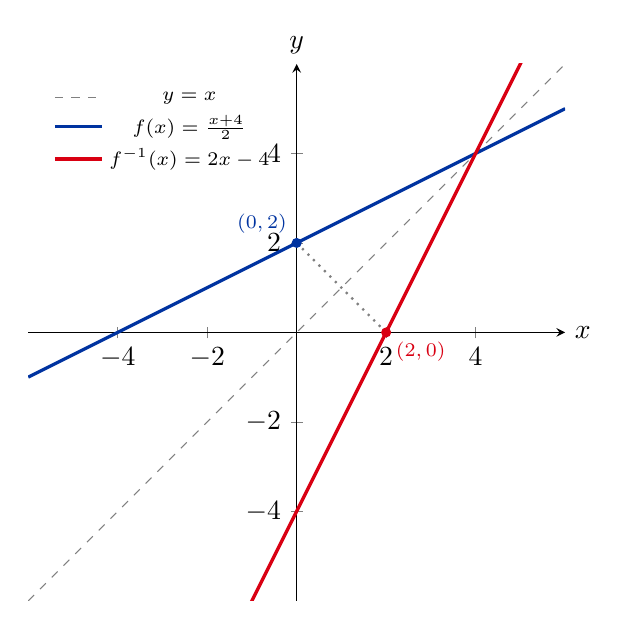
\begin{tikzpicture}
\begin{axis}[
  width=8.4cm, height=8.4cm, axis equal image,
  axis lines=middle, xlabel={$x$}, ylabel={$y$},
  xmin=-6, xmax=6, ymin=-6, ymax=6,
  xtick={-4,-2,2,4}, ytick={-4,-2,2,4},
  legend pos=north west, legend style={font=\scriptsize, draw=none, fill=none},
  every axis x label/.style={at={(ticklabel* cs:1.0)},anchor=west},
  every axis y label/.style={at={(ticklabel* cs:1.0)},anchor=south}]
\addplot[domain=-6:6, samples=2, dashed, gray]{x};
\addlegendentry{$y=x$}
\addplot[domain=-6:6, samples=2, very thick, armBlue]{(x+4)/2};
\addlegendentry{$f(x)=\tfrac{x+4}{2}$}
\addplot[domain=-6:6, samples=2, very thick, armRed]{2*x-4};
\addlegendentry{$f^{-1}(x)=2x-4$}
% a matched pair of mirror points: (0,2) on f, (2,0) on f^{-1}
\addplot[only marks, mark=*, mark size=1.6pt, armBlue] coordinates {(0,2)};
\addplot[only marks, mark=*, mark size=1.6pt, armRed] coordinates {(2,0)};
\draw[dotted, thick, gray] (axis cs:0,2) -- (axis cs:2,0);
\node[font=\scriptsize, armBlue, anchor=south east] at (axis cs:0,2) {$(0,2)$};
\node[font=\scriptsize, armRed, anchor=north west] at (axis cs:2,0) {$(2,0)$};
\end{axis}
\end{tikzpicture}
\end{center}

\begin{methodbox}
\textbf{Փոխանցելի տեխնիկա՝} հակադարձելու համար \emph{լուծիր $y=f(x)$-ը $x$-ի նկատմամբ}։ $\tfrac{ax+b}{cx+d}$
կոտորակի համար խաչաձև բազմապատկիր և բոլոր $x$ անդամները հավաքիր մի կողմ։ Ստուգիր համադրելով՝
$f^{-1}(f(x))$-ը պետք է պարզեցվի $x$-ի։ Հակադարձի գրաֆիկը միշտ $f$-ի արտացոլումն է $y=x$-ի նկատմամբ։
\end{methodbox}

% ============================================================================
\section*{Խնդիր 6 - Ինյեկտիվ, սյուրյեկտիվ, բիյեկտիվ ($f:\R\to\R$)}

\begin{problembox}[6]
Որոշիր, թե $f:\R\to\R$ արտապատկերումներից որոնք են ինյեկտիվ, սյուրյեկտիվ կամ բիյեկտիվ՝
\[
\text{(ա) } |x|,\quad
\text{(բ) } x^2+4,\quad
\text{(գ) } x^3+6,\quad
\text{(դ) } x+|x|,\quad
\text{(ե) } x(x-2)(x+2).
\]
\end{problembox}

\begin{ideabox}
Երկու անկախ հարց, և յուրաքանչյուրն ունի մեկ-տողանի նկար-թեստ։
\textbf{Ինյեկտիվ} («միարժեք») նշանակում է, որ \emph{տարբեր մուտքերը տալիս են տարբեր ելքեր}՝
ոչ մի երկու $x$ արժեք չեն կիսում նույն բարձրությունը։ Նկար-թեստ՝ յուրաքանչյուր \textbf{հորիզոնական
ուղիղ} հատում է գրաֆիկն \emph{առավելագույնը մեկ անգամ}։ Եթե թեկուզ մեկ հորիզոնական ուղիղ կտրում է
գրաֆիկը երկու անգամ, ինյեկտիվությունը ձախողվում է։ \textbf{Սյուրյեկտիվ} («$\R$-ի վրա») նշանակում է, որ
\emph{ամեն} թիրախ-բարձրության հասնում ենք՝ արժեքների տիրույթը ողջ $\R$-ն է։ Նկար-թեստ՝ յուրաքանչյուր
հորիզոնական ուղիղ հատում է գրաֆիկն \emph{առնվազն մեկ անգամ}։ \textbf{Բիյեկտիվ} $=$ երկուսն էլ $=$
յուրաքանչյուր հորիզոնական ուղիղ հատում է \emph{ճիշտ մեկ անգամ} (և այդ դեպքում $f$-ն ունի հակադարձ)։
Դասական մարդասպանները՝ $|x|$-ը կամ զույգ աստիճանը կիսում է ուղիղը երկու մասի (սպանում է
ինյեկտիվությունն ու սյուրյեկտիվությունը)՝ $x^3$-ի նման կենտ աստիճանը մաքուր աճող կոր է (բիյեկտիվ)։
\end{ideabox}

\textbf{Քայլ 1 - Հորիզոնական ուղղի թեստը՝ ֆունկցիա առ ֆունկցիա։}
\begin{itemize}[leftmargin=1.4em,itemsep=1pt]
\item[(ա)] $|x|$՝ $y=1$ ուղիղը հանդիպում է դրան $x=\pm1$-ում (երկու կետ) $\Rightarrow$ \emph{ոչ}
ինյեկտիվ՝ $y=-1$ ուղիղը ոչ մի տեղ չի հանդիպում դրան ($|x|\ge0$) $\Rightarrow$ \emph{ոչ} սյուրյեկտիվ։
\textbf{Ոչ մեկը։}
\item[(բ)] $x^2+4$՝ $f(1)=f(-1)=5$ $\Rightarrow$ ոչ ինյեկտիվ՝ արժեքների տիրույթը $[4,\infty)$ է, ուստի $y=0$-ին
երբեք չենք հասնում $\Rightarrow$ ոչ սյուրյեկտիվ։ \textbf{Ոչ մեկը։}
\item[(գ)] $x^3+6$՝ խիստ աճող է (եթե $x_1<x_2$, ապա $x_1^3<x_2^3$), ուստի յուրաքանչյուր հորիզոնական
ուղիղ հանդիպում է դրան առավելագույնը մեկ անգամ $\Rightarrow$ ինյեկտիվ՝ երբ $x\to\pm\infty$, արժեքն
անցնում է ողջ $\R$-ով, ուստի յուրաքանչյուր ուղիղ հանդիպում է դրան առնվազն մեկ անգամ $\Rightarrow$
սյուրյեկտիվ։ \textbf{Բիյեկտիվ}, հակադարձով $f^{-1}(x)=\sqrt[3]{x-6}$։
\item[(դ)] $x+|x|$՝ $x\le0$-ի համար սա $x+(-x)=0$ է, ուստի ողջ $x\le0$ ճառագայթն արտապատկերվում է $0$-ի
$\Rightarrow$ խիստ ոչ ինյեկտիվ՝ ելքը երբեք բացասական չէ (այն հավասար է $0$-ի կամ $2x>0$-ի)
$\Rightarrow$ արժեքների տիրույթը $[0,\infty)$ է, ոչ սյուրյեկտիվ։ \textbf{Ոչ մեկը։}
\item[(ե)] $x(x-2)(x+2)=x^3-4x$՝ խորանարդ է, ուստի երբ $x\to\pm\infty$, այն ծածկում է ողջ $\R$-ը
$\Rightarrow$ սյուրյեկտիվ՝ բայց $f(0)=f(2)=f(-2)=0$, ուստի $y=0$ ուղիղը հանդիպում է դրան երեք անգամ
$\Rightarrow$ ոչ ինյեկտիվ։ \textbf{Միայն սյուրյեկտիվ։}
\end{itemize}

\textbf{Քայլ 2 - Միշտ ստուգիր վկաները։} Ոչ-ինյեկտիվ վճիռներից յուրաքանչյուրը հենվում է կոնկրետ
բախման վրա՝ $|{-1}|=|1|$, $(-1)^2+4=1^2+4$, $f(-2)=f(0)$ (դ)-ում, և $(-2)(-4)(0)=0=2\cdot0\cdot4$
(ե)-ում։ Ոչ-սյուրյեկտիվ վճիռները հենվում են բաց թողնված թիրախի վրա ($y=-1$ (ա)-ի համար, $y=0$ (բ)/(դ)-ի
համար)։ (գ)-ի համար խորանարդ-արմատի բանաձևն ակնհայտորեն տալիս է նախապատկեր ամեն թիրախի համար։ Ամենը
հաստատված է խիտ ընտրանքով։

\answer{%
(ա) ոչ մեկը;\quad (բ) ոչ մեկը;\quad \textbf{(գ) բիյեկտիվ};\quad
(դ) ոչ մեկը;\quad (ե) սյուրյեկտիվ, բայց ոչ ինյեկտիվ.}

\medskip
\textbf{Ցուցադրությունը՝ սլաք-դիագրամներ և հորիզոնական ուղղի թեստ։} Նախ՝ երեք նկարները,
որ յուրաքանչյուր ուսանող պետք է կրի գլխում։ Ձախ կողմի կետերը մուտքերն են, աջ կողմի կետերը՝
թիրախները՝ սլաքն $x\mapsto f(x)$-ն է։

\begin{center}
\begin{tikzpicture}[font=\scriptsize,>=Stealth,
  dot/.style={circle,fill=ink,inner sep=1.3pt},
  every node/.style={inner sep=1pt}]
\def\dx{2.2}
% --- INJECTIVE not surjective ---
\begin{scope}[shift={(0,0)}]
  \node[font=\small\bfseries] at (1.0,2.5) {Ինյեկտիվ, ոչ վրա};
  \foreach \y/\n in {2/a,1.2/b,0.4/c} {\node[dot] (L\n) at (0,\y) {}; \node[left=2pt of L\n]{$\n$};}
  \foreach \y/\n in {2/p,1.2/q,0.4/r,-0.4/s} {\node[dot] (R\n) at (\dx,\y) {}; \node[right=2pt of R\n,font=\scriptsize]{$\n$};}
  \draw[->,armBlue,thick] (La) -- (Rp);
  \draw[->,armBlue,thick] (Lb) -- (Rq);
  \draw[->,armBlue,thick] (Lc) -- (Rr);
  \node[armRed] at (\dx+0.7,-0.4) {բաց թողնված};
  \node at (0,-1.0) {տարբեր $\to$ տարբեր,};
  \node at (0,-1.4) {բայց $s$-ին չհասանք};
\end{scope}
% --- SURJECTIVE not injective ---
\begin{scope}[shift={(5.0,0)}]
  \node[font=\small\bfseries] at (1.0,2.5) {Վրա, ոչ ինյեկտիվ};
  \foreach \y/\n in {2/a,1.2/b,0.4/c,-0.4/d} {\node[dot] (L\n) at (0,\y) {};}
  \foreach \y/\n in {1.6/p,0.6/q} {\node[dot] (R\n) at (\dx,\y) {};}
  \draw[->,armBlue,thick] (La) -- (Rp);
  \draw[->,armRed,thick]  (Lb) -- (Rp);
  \draw[->,armBlue,thick] (Lc) -- (Rq);
  \draw[->,armRed,thick]  (Ld) -- (Rq);
  \node at (0,-1.0) {ամեն թիրախին հասանք,};
  \node at (0,-1.4) {բայց երկու սլաք բախվում են};
\end{scope}
% --- BIJECTIVE ---
\begin{scope}[shift={(10.0,0)}]
  \node[font=\small\bfseries] at (1.0,2.5) {Բիյեկտիվ};
  \foreach \y/\n in {2/a,1.2/b,0.4/c} {\node[dot] (L\n) at (0,\y) {};}
  \foreach \y/\n in {2/p,1.2/q,0.4/r} {\node[dot] (R\n) at (\dx,\y) {};}
  \draw[->,armBlue,thick] (La) -- (Rp);
  \draw[->,armBlue,thick] (Lb) -- (Rq);
  \draw[->,armBlue,thick] (Lc) -- (Rr);
  \node at (0,-1.0) {կատարյալ զուգակցում՝};
  \node at (0,-1.4) {մեկ սլաք ներս, մեկը՝ դուրս};
\end{scope}
\end{tikzpicture}
\end{center}

Հիմա հորիզոնական ուղղի թեստը կիրառված այս խնդրի երկու հակադրվող գրաֆիկներին՝ $x^2+4$
(ծալված, ուղիղը կարող է երկու անգամ կտրել) ընդդեմ $x^3+6$ (միապաղաղ, յուրաքանչյուր ուղիղ կտրում է ճիշտ
մեկ անգամ)։

\begin{center}
\begin{tikzpicture}
\begin{axis}[
  name=p1, width=7.2cm, height=5.6cm, axis lines=middle,
  xlabel={$x$}, ylabel={$y$}, xmin=-3.2, xmax=3.2, ymin=-1, ymax=12,
  title={(բ) $x^2+4$՝ $y=5$ ուղիղը կտրում է երկու անգամ}, title style={font=\scriptsize},
  every axis x label/.style={at={(ticklabel* cs:1.0)},anchor=west},
  every axis y label/.style={at={(ticklabel* cs:1.0)},anchor=south}]
\addplot[domain=-2.8:2.8, samples=80, very thick, armBlue]{x^2+4};
\addplot[domain=-3.2:3.2, samples=2, armRed, thick]{5};
\addplot[only marks, mark=*, mark size=1.4pt, armRed] coordinates {(-1,5)(1,5)};
\node[font=\scriptsize, armRed, anchor=south] at (axis cs:0,5.1) {$y=5$};
\end{axis}
\begin{axis}[
  name=p2, at={($(p1.east)+(1.8cm,0)$)}, anchor=west,
  width=7.2cm, height=5.6cm, axis lines=middle,
  xlabel={$x$}, ylabel={$y$}, xmin=-3, xmax=3, ymin=-12, ymax=18,
  title={(գ) $x^3+6$՝ յուրաքանչյուր ուղիղ կտրում է մեկ անգամ}, title style={font=\scriptsize},
  every axis x label/.style={at={(ticklabel* cs:1.0)},anchor=west},
  every axis y label/.style={at={(ticklabel* cs:1.0)},anchor=south}]
\addplot[domain=-2.6:2.6, samples=80, very thick, armBlue]{x^3+6};
\addplot[domain=-3:3, samples=2, armRed, thick]{2};
\addplot[domain=-3:3, samples=2, armOrange, thick]{13};
\addplot[only marks, mark=*, mark size=1.4pt, ink] coordinates {(-1.587,2)(1.913,13)};
\node[font=\scriptsize, armRed, anchor=south] at (axis cs:-2.2,2.4) {$y=2$};
\node[font=\scriptsize, armOrange!75!black, anchor=south] at (axis cs:-2.4,13.4) {$y=13$};
\end{axis}
\end{tikzpicture}
\end{center}

\begin{methodbox}
\textbf{Փոխանցելի տեխնիկա՝} ինյեկտիվությունը հերքելու համար ցույց տուր մեկ բախում $f(a)=f(b)$՝
$a\ne b$-ով։ Սյուրյեկտիվությունը հերքելու համար ցույց տուր մեկ չհասած թիրախ։ Իրական ֆունկցիայի
բիյեկտիվությունն ապացուցելու համար ցույց տուր, որ այն խիստ միապաղաղ է (ինյեկտիվ) և անցնում է
$-\infty$-ից $+\infty$ (սյուրյեկտիվ)՝ ապա այն ունի հակադարձ։ Զույգ աստիճանները և $|x|$-ը ծալում են՝
կենտ աստիճանները՝ ոչ։
\end{methodbox}

% ============================================================================
\section*{Խնդիր 10 - $\Ker(f)$-ը համարժեքության հարաբերություն է}

\begin{problembox}[10]
Ցույց տուր, որ ցանկացած $f:A\to B$ ֆունկցիայի համար նրա \textbf{միջուկը}
$\Ker(f)=\{(x,y)\in A\times A: f(x)=f(y)\}$ համարժեքության հարաբերություն է $A$-ի վրա։
\end{problembox}

\begin{ideabox}
Միջուկը կապում է երկու մուտք հենց այն ժամանակ, երբ դրանք ունեն \emph{նույն ելքը}։ Բայց «նույն
արժեքն ունենալը» կառուցված է ուղիղ այդ արժեքների \emph{հավասարությունից} ($=$), իսկ հավասարությունն
ամենահամարժեքության-նման հարաբերությունն է, որ կա՝ ամեն ինչ հավասար է ինքն իրեն, հավասարությունը
սիմետրիկ է, և այն շղթայվում է։ Ուստի $\Ker(f)$-ը ժառանգում է $=$-ի բոլոր երեք հատկությունները
ձրիաբար։ Շահող պատկերը՝ $\Ker(f)$-ը կտրում է որոշման տիրույթը \textbf{շերտերի}, մեկ կույտ ելքի ամեն
արժեքի համար, որտեղ $f^{-1}(b)$ շերտը բոլոր այն մուտքերն են, որ $f$-ն ուղարկում է $b$-ի։
Համարժեքության դասերը $=$ շերտեր։
\end{ideabox}

\textbf{Քայլ 1 - Ռեֆլեքսիվ։} Ցանկացած $x\in A$-ի համար $f(x)=f(x)$ ակնհայտորեն, ուստի $(x,x)\in\Ker(f)$։

\textbf{Քայլ 2 - Սիմետրիկ։} Եթե $(x,y)\in\Ker(f)$, ապա $f(x)=f(y)$՝ հավասարությունը սիմետրիկ է, ուստի
$f(y)=f(x)$, հետևաբար $(y,x)\in\Ker(f)$։

\textbf{Քայլ 3 - Փոխանցական։} Եթե $(x,y),(y,z)\in\Ker(f)$, ապա $f(x)=f(y)$ և $f(y)=f(z)$՝ հավասարությունները
շղթայելով՝ $f(x)=f(z)$, հետևաբար $(x,z)\in\Ker(f)$։

\textbf{Քայլ 4 - Եզրակացություն և շերտերի պատկերը։} Բոլոր երեքն էլ տեղի ունեն, ուստի $\Ker(f)$-ը
համարժեքության հարաբերություն է։ $x$-ի համարժեքության դասն է $\{y:f(y)=f(x)\}=f^{-1}(f(x))$՝ շերտը
$f(x)$ արժեքի վրա։ Այս շերտերը տրոհում են $A$-ն՝ ամեն մուտք ընկնում է ճիշտ մեկ շերտում (իր սեփական
ելքը), և տարբեր ելքի արժեքները տալիս են չհատվող շերտեր։

\answer{$\Ker(f)$-ը ռեֆլեքսիվ է, սիմետրիկ և փոխանցական ($B$-ի վրա $=$-ից ժառանգված), հետևաբար
համարժեքության հարաբերություն է $A$-ի վրա՝ նրա դասերը $f^{-1}(b)$ շերտերն են։}

\medskip
\textbf{Շերտերի տրոհումը։} Վերցրու խաղալիք արտապատկերումը $f:\{1,2,3,4,5,6\}\to\{p,q,r\}$՝
$f(1)=f(2)=f(3)=p$, $f(4)=f(5)=q$, $f(6)=r$։ Միջուկը տրոհում է որոշման տիրույթը երեք շերտի,
մեկ՝ ամեն արժեքի համար։ Երկու մուտք $\Ker(f)$-կապված են այն և միայն այն դեպքում, երբ նստած են նույն
ստվերավորված կույտում։

\begin{center}
\begin{tikzpicture}[font=\small,>=Stealth,
  dot/.style={circle,fill=ink,inner sep=1.6pt}]
% domain A with three fibers
\begin{scope}
  \node[draw,rounded corners,fill=armBlue!12,minimum width=1.7cm,minimum height=2.5cm] (f1) at (0,0) {};
  \node[draw,rounded corners,fill=armRed!12,minimum width=1.7cm,minimum height=1.9cm] (f2) at (2.2,-0.3) {};
  \node[draw,rounded corners,fill=armOrange!18,minimum width=1.7cm,minimum height=1.2cm] (f3) at (4.4,-0.65) {};
  \node[dot,label=left:$1$] (n1) at (-0.4,0.7) {};
  \node[dot,label=left:$2$] (n2) at (-0.4,0.0) {};
  \node[dot,label=left:$3$] (n3) at (-0.4,-0.7) {};
  \node[dot,label=left:$4$] (n4) at (1.8,0.2) {};
  \node[dot,label=left:$5$] (n5) at (1.8,-0.6) {};
  \node[dot,label=left:$6$] (n6) at (4.0,-0.65) {};
  \node[font=\scriptsize] at (0,-1.5) {շերտ $p$-ի վրա};
  \node[font=\scriptsize] at (2.2,-1.5) {շերտ $q$-ի վրա};
  \node[font=\scriptsize] at (4.4,-1.5) {շերտ $r$-ի վրա};
  \node[font=\small\itshape] at (2.2,1.7) {որոշման տիրույթ $A$՝ $\Ker(f)$-ով տրոհված};
\end{scope}
% codomain B
\begin{scope}[shift={(8.6,0)}]
  \node[dot,label=right:$p$] (bp) at (0,0.7) {};
  \node[dot,label=right:$q$] (bq) at (0,0.0) {};
  \node[dot,label=right:$r$] (br) at (0,-0.7) {};
  \node[font=\small\itshape] at (0.1,1.7) {$B$};
\end{scope}
% arrows
\draw[->,armBlue]   (n1) to[out=0,in=170] (bp);
\draw[->,armBlue]   (n2) to[out=0,in=175] (bp);
\draw[->,armBlue]   (n3) to[out=0,in=185] (bp);
\draw[->,armRed]    (n4) to[out=0,in=170] (bq);
\draw[->,armRed]    (n5) to[out=0,in=190] (bq);
\draw[->,armOrange!80!black] (n6) to[out=0,in=200] (br);
\end{tikzpicture}
\end{center}

\begin{methodbox}
\textbf{Փոխանցելի տեխնիկա՝} ցանկացած «$x\sim y$ այն և միայն այն դեպքում, երբ
$g(x)=g(y)$» («ինչ-որ մեծության նույն արժեքը») ձևի հարաբերություն ինքնաբերաբար համարժեքության
հարաբերություն է, քանի որ այն հետ է քաշված $=$-ից։ Նրա դասերն $g$-ի մակարդակային բազմություններն /
շերտերն են։ Սա ամենատարածված եղանակն է, որով համարժեքության հարաբերություններն առաջանում են։
\end{methodbox}

% ============================================================================
\section*{Խնդիր 12 - $f(x)=\dfrac{x}{2x+1}$-ը $\Q^+$-ի վրա ինյեկտիվ է, բայց ոչ սյուրյեկտիվ}

\begin{problembox}[12]
Դիցուք $f:\Q^+\to\Q^+$ լինի $f(x)=\dfrac{x}{2x+1}$։ Ցույց տուր, որ $f$-ն ինյեկտիվ է, բայց ոչ սյուրյեկտիվ։
\end{problembox}

\begin{ideabox}
\textbf{Ինյեկտիվությունը} մաքուր հանրահաշիվ է՝ ենթադրիր, որ երկու մուտք տալիս են նույն ելքը, և մանրացրու
հավասարումը, մինչև այն հարկադրի, որ մուտքերը հավասար լինեն։ \textbf{Ոչ սյուրյեկտիվությունը} պահանջում
է թիրախ առանց նախապատկերի, և այն գտնելու մաքուր եղանակը արժեքների տիրույթը \emph{սահմանափակելն} է։
Դրական $x$-ի համար հայտարարը $2x+1$-ը մի փոքր մեծ է $2x$-ից, ուստի $\tfrac{x}{2x+1}$-ը մի փոքր փոքր է
$\tfrac{x}{2x}=\tfrac12$-ից։ Ուստի ամեն ելք խստորեն ցածր է $\tfrac12$-ից։ Այսպիսով, $\ge\tfrac12$ ամեն
ինչ (օրինակ՝ $1$ արժեքը, որ $\Q^+$-ում է) անհասանելի է՝ սյուրյեկտիվությունը ձախողվում է մեծ լայնքով։
\end{ideabox}

\textbf{Քայլ 1 - Ինյեկտիվ։} Ենթադրիր $f(x)=f(y)$, այսինքն $\dfrac{x}{2x+1}=\dfrac{y}{2y+1}$։
Խաչաձև բազմապատկիր (երկու հայտարարներն էլ դրական են)՝ $x(2y+1)=y(2x+1)$, ուստի $2xy+x=2xy+y$, հետևաբար
$x=y$։ Տարբեր մուտքերը չեն կարող կիսել նույն ելքը, ուստի $f$-ն ինյեկտիվ է։

\textbf{Քայլ 2 - Սահմանափակիր արժեքների տիրույթը։} $x\in\Q^+$-ի համար ունենք $x>0$, ուստի $2x+1>2x>0$ և
հետևաբար
\[
f(x)=\frac{x}{2x+1}<\frac{x}{2x}=\frac12.
\]
Նաև $f(x)>0$։ Ուստի ողջ արժեքների տիրույթը նստած է $\bigl(0,\tfrac12\bigr)$ բաց միջակայքի ներսում։

\textbf{Քայլ 3 - Ցույց տուր բաց թողնված թիրախ։} $1\in\Q^+$ թիվը բավարարում է $1\ge\tfrac12$, ուստի այն
$(0,\tfrac12)$-ից դուրս է և չի կարող լինել $f$-ի արժեք։ (Հանրահաշվորեն՝ $\tfrac{x}{2x+1}=1$ հարկադրում է
$x=2x+1$, այսինքն $x=-1\notin\Q^+$։) Հետևաբար $f$-ն \emph{ոչ} սյուրյեկտիվ է։

\textbf{Քայլ 4 - Միշտ ստուգիր, որ սահմանը խիստ է, բայց երբեք չի հասնում։} Երբ $x\to\infty$,
$f(x)=\tfrac{x}{2x+1}\to\tfrac12$ ներքևից (օրինակ՝ $f(10000)\approx0.49998$), ուստի $\tfrac12$-ը
սուպրեմումն է, բայց նույնպես երբեք չի հասնում՝ հաստատելով, որ արժեքների տիրույթը խստորեն $(0,\tfrac12)$-ի
ներսում է։

\answer{Ինյեկտիվ՝ $f(x)=f(y)\Rightarrow x=y$։ Ոչ սյուրյեկտիվ՝ ամեն արժեք $<\tfrac12$ է, ուստի օրինակ
$1$-ը (և $\ge\tfrac12$ ամեն արժեք) նախապատկեր չունի։}

\medskip
\textbf{Արժեքների տիրույթը նստած է $y=\tfrac12$-ից ցածր։} $f$-ը $x>0$-ի համար գծագրելով՝ կորը բարձրանում է
$0$-ից, բայց հավերժ մնում է կետագիծ առաստաղի $y=\tfrac12$-ի տակ։ $\Q^+$-ի ողջ թիրախ-գոտին
$\bigl[\tfrac12,\infty\bigr)$՝ ներառյալ $1$-ը՝ դատարկ է արժեքներից։

\begin{center}
\begin{tikzpicture}
\begin{axis}[
  width=12cm, height=6.2cm, axis lines=middle,
  xlabel={$x$}, ylabel={$y=f(x)$}, xmin=-0.3, xmax=12, ymin=-0.05, ymax=0.78,
  ytick={0.5}, yticklabels={$\tfrac12$}, xtick={0,2,4,6,8,10},
  every axis x label/.style={at={(ticklabel* cs:1.0)},anchor=west},
  every axis y label/.style={at={(ticklabel* cs:1.0)},anchor=south}]
% horizontal asymptote / ceiling
\addplot[domain=0:12, samples=2, dashed, armRed, thick]{0.5};
\node[font=\scriptsize, armRed, anchor=south west] at (axis cs:8.2,0.5) {առաստաղ $y=\tfrac12$ (երբեք չի հասնում)};
% the function
\addplot[domain=0.001:12, samples=200, very thick, armBlue]{x/(2*x+1)};
% the unreachable band sits at and above the ceiling y=1/2
\node[font=\scriptsize, anchor=west] at (axis cs:0.4,0.66) {անհասանելի թիրախ-գոտի՝ բոլոր $y\ge\tfrac12$ (օր.\ $y=1$)};
\node[font=\scriptsize, armBlue, anchor=west] at (axis cs:6,0.40) {արժ. տիրույթ $\subset(0,\tfrac12)$};
\end{axis}
\end{tikzpicture}
\end{center}

\begin{methodbox}
\textbf{Փոխանցելի տեխնիկա՝} «ոչ սյուրյեկտիվ» ցույց տալու համար \emph{սահմանափակիր արժեքների տիրույթը} և
անվանիր մեկ թիրախ՝ սահմանից դուրս։ $\tfrac{x}{2x+1}<\tfrac{x}{2x}$ գնահատականը (փոքրացրու հայտարարի
$+1$-ը) ռացիոնալ ֆունկցիաների բանվոր հնարքն է։ Հարաբերության ինյեկտիվությունը սովորաբար մեկ-տողանի
խաչաձև բազմապատկում է։
\end{methodbox}

% ============================================================================
\section*{Խնդիր 19 - Ե՞րբ է $f(A\cap B)=f(A)\cap f(B)$}

\begin{problembox}[19]
Որ ֆունկցիաների համար է $f(A\cap B)=f(A)\cap f(B)$ տեղի ունենում բոլոր $A,B$ բազմությունների համար։
\end{problembox}

\begin{ideabox}
Մեկ պարունակումը ձրի է, մյուսն ինյեկտիվություն արժե։ \emph{Ձրի ուղղություն}՝ եթե $x\in A\cap B$, ապա
$f(x)$-ը և՛ $f(A)$-ում է, և՛ $f(B)$-ում, ուստի $f(A\cap B)\subseteq f(A)\cap f(B)$ \emph{միշտ}։
Հակառակը կարող է ձախողվել, որովհետև $f(A)\cap f(B)$-ն հավաքում է \textbf{ընդհանուր ելքի արժեքները},
որոնք կարող են գալ \emph{տարբեր} մուտքերից՝ մեկ մուտք $A$-ում, մյուսը՝ $B$-ում՝ որոնք պարտադիր չէ, որ
հանդիպեն $A\cap B$-ում։ Հենց երբ $f$-ն \textbf{ինյեկտիվ} է, ընդհանուր ելքը հարկադրում է ընդհանուր
մուտք, և երկու կողմերը դառնում են հավասար։ Ուստի նույնությունը տեղի ունի բոլոր $A,B$-ի համար \textbf{այն
և միայն այն դեպքում, երբ $f$-ն ինյեկտիվ է}։
\end{ideabox}

\textbf{Քայլ 1 - Միշտ ճիշտ պարունակումը։} Դիցուք $y\in f(A\cap B)$, ուստի $y=f(x)$՝ $x\in A\cap B$-ով։
Ապա $x\in A$ տալիս է $y\in f(A)$, և $x\in B$ տալիս է $y\in f(B)$, ուստի $y\in f(A)\cap f(B)$։
Հետևաբար $f(A\cap B)\subseteq f(A)\cap f(B)$ \emph{ամեն} $f$-ի համար։

\textbf{Քայլ 2 - Եթե $f$-ն ինյեկտիվ է, հակառակը տեղի ունի։} Դիցուք $y\in f(A)\cap f(B)$, ուստի
$y=f(a)=f(b)$՝ $a\in A$-ով և $b\in B$-ով։ Ինյեկտիվությունը հարկադրում է $a=b$, և այս ընդհանուր կետը
ընկած է $A\cap B$-ում։ Այսպիսով $y=f(a)\in f(A\cap B)$։ Ուստի $f(A)\cap f(B)\subseteq f(A\cap B)$, և
Քայլ 1-ի հետ զուգակցելով՝ ստանում ենք հավասարություն։

\textbf{Քայլ 3 - Եթե $f$-ն ինյեկտիվ չէ, նույնությունը ձախողվում է որոշ $A,B$-ի համար։} Ընտրիր $a\ne a'$՝
$f(a)=f(a')$-ով, և դիր $A=\{a\}$, $B=\{a'\}$։ Ապա $A\cap B=\varnothing$, ուստի $f(A\cap B)=\varnothing$,
բայց $f(A)\cap f(B)=\{f(a)\}\cap\{f(a')\}=\{f(a)\}\ne\varnothing$։ Նույնությունը կոտրվում է։

\textbf{Քայլ 4 - Միշտ ստուգիր կոնկրետ արտապատկերման վրա։} $f(x)=x^2$, $A=\{1\}$, $B=\{-1\}$՝
$f(A\cap B)=f(\varnothing)=\varnothing$, բայց $f(A)\cap f(B)=\{1\}\cap\{1\}=\{1\}$։ Խիստ ճեղքը
տեսանելի է, և դա հենց ոչ-ինյեկտիվությունն է ($1\neq-1$, բայց $f(1)=f(-1)$), որ բացում է այն՝ ինյեկտիվ
$f$-ի համար Քայլ 2-ը հարկադրում է հավասարություն։

\answer{Հենց \textbf{ինյեկտիվ} ֆունկցիաները։ $\subseteq$ պարունակումը միշտ տեղի ունի՝ հավասարությունը
տեղի ունի բոլոր $A,B$-ի համար այն և միայն այն դեպքում, երբ $f$-ն ինյեկտիվ է։}

\medskip
\textbf{Ինչու՞ է ոչ-ինյեկտիվությունը կոտրում այն։} Երկու տարբեր մուտքեր $a\in A$ և $a'\in B$ փլվում են
\emph{նույն} ելքին $v$։ Այդ ելքն ընկնում է և՛ $f(A)$-ում, և՛ $f(B)$-ում, ուստի այն նստած է
հատման մեջ աջ կողմում՝ թեև $A$-ն և $B$-ն ընդհանրապես ոչ մի մուտք չեն կիսում՝ թողնելով $f(A\cap B)$-ն
դատարկ։

\begin{center}
\begin{tikzpicture}[font=\small,>=Stealth, dot/.style={circle,fill=ink,inner sep=1.6pt}]
% set A
\node[draw,ellipse,fill=armBlue!12,minimum width=2.4cm,minimum height=1.5cm] (A) at (0,1.1) {};
\node[font=\scriptsize,armBlue] at (-1.5,1.1) {$A$};
\node[dot,label=above:$a$] (a) at (0,1.1) {};
% set B
\node[draw,ellipse,fill=armRed!12,minimum width=2.4cm,minimum height=1.5cm] (B) at (0,-0.9) {};
\node[font=\scriptsize,armRed] at (-1.5,-0.9) {$B$};
\node[dot,label=below:$a'$] (b) at (0,-0.9) {};
\node[font=\scriptsize] at (0,0.1) {$A\cap B=\varnothing$};
% shared output
\node[dot,label={right:$v=f(a)=f(a')$}] (v) at (5.2,0.1) {};
\node[font=\scriptsize] at (5.2,1.1) {փոփոխման տիրույթ};
\draw[->,armBlue,thick] (a) to[out=0,in=120] (v);
\draw[->,armRed,thick]  (b) to[out=0,in=240] (v);
\node[font=\scriptsize] at (5.4,-0.6) {$v\in f(A)\cap f(B)$};
\node[font=\scriptsize] at (5.4,-1.1) {բայց $v\notin f(A\cap B)=\varnothing$};
\end{tikzpicture}
\end{center}

\begin{methodbox}
\textbf{Փոխանցելի տեխնիկա՝} պատկերի օրենքների համար այն պարունակումը, որ վարկած չի պահանջում, միշտ
«հատման պատկերը $\subseteq$ պատկերների հատում»-ն է։ Հակառակը պահանջում է ինյեկտիվություն, և
հակառակ օրինակը միշտ տարբեր եզակիների մեջ տեղադրված երկու բախման կետ է։ (Միավորումն ավելի լավ է
պահվում՝ $f(A\cup B)=f(A)\cup f(B)$ \emph{ամեն} $f$-ի համար։)
\end{methodbox}

% ============================================================================
\section*{Խնդիր 22 - Կարո՞ղ են չհատվող ոչ դատարկ $X_1,X_2$ ունենալ $f(X_1)=f(X_2)$}

\begin{problembox}[22]
$f:A\to B$-ի և չհատվող ոչ դատարկ $X_1,X_2\subseteq A$-ի համար (ուստի $X_1\cap X_2=\varnothing$),
\emph{կարո՞ղ} են պատկերները հավասար լինել՝ $f(X_1)=f(X_2)$։
\end{problembox}

\begin{ideabox}
Պատկերները ելքի \emph{արժեքների} մասին են, ոչ թե այն մասին, թե որ մուտքերն են դրանք արտադրել։ Երկու
բոլորովին առանձին մուտքի բազմություններ կարող են, այնուամենայնիվ, հասնել ճիշտ նույն ելքերի
բազմությանը, պայմանով, որ $f$-ն իրար սոսնձի դրանց կետերը։ Ուստի հենց որ $f$-ն ոչ ինյեկտիվ է,
պատասխանը \textbf{այո է, հավասար պատկերները հնարավոր են}։ (Նկատի առ հարցի ամենամաքուր ընթերցումը՝
հավասար պատկերներ \emph{հարկադրված} չեն՝ վերցրու $X_1=\{1\}$, $X_2=\{2\}$ նույնական արտապատկերման տակ՝
անհավասար պատկերներ ստանալու համար, բայց դրանք \emph{կարող են} պատահել, ինչը հետաքրքրական
բովանդակությունն է։)
\end{ideabox}

\textbf{Քայլ 1 - Կառուցիր օրինակ։} Վերցրու $f:\R\to\R$, $f(x)=x^2$, և չհատվող եզակիները
$X_1=\{1\}$, $X_2=\{-1\}$։ Դրանք ոչ դատարկ են, և $X_1\cap X_2=\varnothing$։

\textbf{Քայլ 2 - Հաշվիր պատկերները։} $f(X_1)=\{1^2\}=\{1\}$ և $f(X_2)=\{(-1)^2\}=\{1\}$։ Ուստի
$f(X_1)=f(X_2)=\{1\}$՝ հավասար պատկերներ չհատվող բազմություններից։

\textbf{Քայլ 3 - Միշտ ստուգիր տրամաբանությունը։} Հնարքը հենց ոչ-ինյեկտիվությունն է՝ $f$-ն ուղարկում է
տարբեր $1$ և $-1$ կետերը նույն արժեքին։ Ավելի մեծ օրինակով՝ $X_1=\{1,2\}$,
$X_2=\{-1,-2\}$ տալիս է $f(X_1)=\{1,4\}=f(X_2)$ նույնպես։ (Եթե $f$-ն \emph{ինյեկտիվ} \emph{լիներ},
չհատվող ոչ դատարկ բազմությունները միշտ կունենային անհավասար՝ իրականում չհատվող՝ պատկերներ։)

\answer{\textbf{Այո}, հնարավոր է։ Օրինակ՝ $f(x)=x^2$, $X_1=\{1\}$, $X_2=\{-1\}$ չհատվող են, սակայն
$f(X_1)=f(X_2)=\{1\}$։ (Հավասար պատկերները հարկադրված չեն, բայց կարող են պատահել, երբ $f$-ն ոչ
ինյեկտիվ է։)}

\medskip
\textbf{Պատկեր՝ երկու չհատվող բազմություն, մեկ ընդհանուր պատկեր։} $f(x)=x^2$-ի սլաք-դիագրամը
$\{-2,-1,1,2\}$-ի վրա՝ սիմետրիկ զույգերը $\{1,2\}$-ը և $\{-1,-2\}$-ը արտապատկերվում են նույն արժեքների
բազմությանը $\{1,4\}$։

\begin{center}
\begin{tikzpicture}[font=\small,>=Stealth, dot/.style={circle,fill=ink,inner sep=1.6pt}]
\node[draw,rounded corners,fill=armBlue!12,minimum width=1.4cm,minimum height=1.7cm] at (0,1.2) {};
\node[font=\scriptsize,armBlue] at (-1.2,1.2) {$X_1$};
\node[dot,label=left:$1$] (p1) at (0,1.6) {};
\node[dot,label=left:$2$] (p2) at (0,0.8) {};
\node[draw,rounded corners,fill=armRed!12,minimum width=1.4cm,minimum height=1.7cm] at (0,-1.2) {};
\node[font=\scriptsize,armRed] at (-1.2,-1.2) {$X_2$};
\node[dot,label=left:$-1$] (m1) at (0,-0.8) {};
\node[dot,label=left:$-2$] (m2) at (0,-1.6) {};
\node[draw,rounded corners,fill=armOrange!18,minimum width=1.4cm,minimum height=1.7cm] at (5,0) {};
\node[font=\scriptsize] at (6.0,0.9) {ընդհանուր պատկեր $\{1,4\}$};
\node[dot,label=right:$1$] (v1) at (5,0.4) {};
\node[dot,label=right:$4$] (v2) at (5,-0.4) {};
\draw[->,armBlue,thick] (p1) to[out=0,in=160] (v1);
\draw[->,armBlue,thick] (p2) to[out=0,in=170] (v2);
\draw[->,armRed,thick]  (m1) to[out=0,in=200] (v1);
\draw[->,armRed,thick]  (m2) to[out=0,in=190] (v2);
\end{tikzpicture}
\end{center}

\begin{methodbox}
\textbf{Փոխանցելի տեխնիկա՝} «բազմության պատկերը» մոռանում է պատիկությունը և ծագումը։ Երբ որևէ
հատկություն միայն պատկերների մասին է, ոչ-ինյեկտիվ $f$-ը (ծալող արտապատկերում՝ $x^2$-ի կամ $|x|$-ի նման)
անակնկալների քո գնալիք աղբյուրն է։
\end{methodbox}

% ============================================================================
\section*{Խնդիր 24 - Արդյո՞ք $Y_1\cap Y_2=\varnothing$-ը հարկադրում է $f^{-1}(Y_1)\cap f^{-1}(Y_2)=\varnothing$}

\begin{problembox}[24]
Ճի՞շտ է, որ $f:A\to B$-ի և $Y_1,Y_2\subseteq B$-ի համար, եթե $Y_1\cap Y_2=\varnothing$, ապա
$f^{-1}(Y_1)\cap f^{-1}(Y_2)=\varnothing$։
\end{problembox}

\begin{ideabox}
Նախապատկերներն իրենց պահում են \emph{կատարյալ}՝ պատկերներից շատ ավելի լավ՝ քանի որ ամեն մուտք $x$ ունի
ճիշտ \emph{մեկ} ելք $f(x)$, ուստի «արդյո՞ք $x$-ը $f^{-1}(Y)$-ում է» հարցնելը պարզապես «արդյո՞ք
միակ արժեքը $f(x)$-ը $Y$-ում է» հարցնելն է։ Եթե $x$-ը երկու նախապատկերներում էլ լիներ, միակ արժեքը
$f(x)$-ը ստիպված կլիներ ապրել և՛ $Y_1$-ում, և՛ $Y_2$-ում միաժամանակ՝ անհնարին, երբ դրանք չհատվող
են։ Ինյեկտիվություն պետք չէ՝ սա \textbf{միշտ} ճիշտ է։ Ավելի խորը փաստն այն է, որ
$f^{-1}(Y_1)\cap f^{-1}(Y_2)=f^{-1}(Y_1\cap Y_2)$ ամեն $f$-ի համար։
\end{ideabox}

\textbf{Քայլ 1 - Ենթադրիր, որ հատումը ոչ դատարկ է, և բեր հակասության։} Դիցուք
$x\in f^{-1}(Y_1)\cap f^{-1}(Y_2)$։ Ապա $f(x)\in Y_1$ և $f(x)\in Y_2$, ուստի
$f(x)\in Y_1\cap Y_2$։

\textbf{Քայլ 2 - Օգտագործիր չհատվածությունը։} Բայց $Y_1\cap Y_2=\varnothing$, ուստի $f(x)$-ը պատկանում է
դատարկ բազմությանը՝ անհնարին։ Հետևաբար այդպիսի $x$ գոյություն չունի, և
$f^{-1}(Y_1)\cap f^{-1}(Y_2)=\varnothing$։

\textbf{Քայլ 3 - Մաքուր պատճառը (ընդհանուր նույնություն)։} Ցանկացած $x$-ի համար՝
\[
x\in f^{-1}(Y_1)\cap f^{-1}(Y_2)
\iff f(x)\in Y_1 \text{ և } f(x)\in Y_2
\iff f(x)\in Y_1\cap Y_2
\iff x\in f^{-1}(Y_1\cap Y_2).
\]
Ուստի $f^{-1}(Y_1)\cap f^{-1}(Y_2)=f^{-1}(Y_1\cap Y_2)$ \emph{միշտ}, և չհատվող դեպքը
հատուկ դեպքն է՝ $Y_1\cap Y_2=\varnothing\Rightarrow f^{-1}(\varnothing)=\varnothing$։

\textbf{Քայլ 4 - Միշտ ստուգիր կոնկրետ արտապատկերման վրա։} Քայլ 3-ը ապացուցում է նույնությունն ամեն $f$-ի
համար՝ $f(x)=x^2$-ով կոնկրետ դեպքը ($Y_1=\{1\}$, $Y_2=\{4\}$՝ տալով չհատվող նախապատկերներ
$\{\pm1\},\{\pm2\}$, որոնց միավորումը $f^{-1}(\{1,4\})$ է) հաստատում է և՛ նույնությունը
$f^{-1}(Y_1)\cap f^{-1}(Y_2)=f^{-1}(Y_1\cap Y_2)$, և՛ չհատվող հետևանքը։

\answer{\textbf{Այո, միշտ} ($f$-ի վրա վարկած պետք չէ)։ Իրականում
$f^{-1}(Y_1)\cap f^{-1}(Y_2)=f^{-1}(Y_1\cap Y_2)$, ուստի չհատվող $Y$-երը տալիս են չհատվող նախապատկերներ։}

\medskip
\textbf{Ինչու՞ նախապատկերները չեն կարող այստեղ համընկնել։} Ամեն մուտք ունի միակ ելք, ուստի այն կարող է
նստել միայն այն թիրախ-բլոկի նախապատկերում, որ պարունակում է այդ միակ արժեքը։ Չհատվող թիրախ-բլոկներ
$\Rightarrow$ ամեն մուտք պարտավորված է առավելագույնը մեկին $\Rightarrow$ ոչ մի մուտք չի կիսվում։

\begin{center}
\begin{tikzpicture}[font=\small,>=Stealth, dot/.style={circle,fill=ink,inner sep=1.5pt}]
% domain
\node[draw,rounded corners,fill=gray!10,minimum width=2cm,minimum height=3.2cm] at (0,0) {};
\node[font=\scriptsize] at (0,1.9) {որոշման տիրույթ $A$};
\node[dot,label=left:$x_1$] (x1) at (-0.1,1.0) {};
\node[dot,label=left:$x_2$] (x2) at (-0.1,0.2) {};
\node[dot,label=left:$x_3$] (x3) at (-0.1,-0.6) {};
\node[dot,label=left:$x_4$] (x4) at (-0.1,-1.4) {};
% codomain with two disjoint blocks
\node[draw,rounded corners,fill=armBlue!12,minimum width=1.6cm,minimum height=1.4cm] at (5,0.9) {};
\node[font=\scriptsize,armBlue] at (5,1.75) {$Y_1$};
\node[draw,rounded corners,fill=armRed!12,minimum width=1.6cm,minimum height=1.4cm] at (5,-0.9) {};
\node[font=\scriptsize,armRed] at (5,-1.75) {$Y_2$};
\node[dot] (u1) at (5,1.2) {};
\node[dot] (u2) at (5,0.5) {};
\node[dot] (u3) at (5,-0.6) {};
\node[dot] (u4) at (5,-1.2) {};
\draw[->,armBlue,thick] (x1) -- (u1);
\draw[->,armBlue,thick] (x2) -- (u2);
\draw[->,armRed,thick]  (x3) -- (u3);
\draw[->,armRed,thick]  (x4) -- (u4);
\node[font=\scriptsize,armBlue,anchor=west] at (-1.4,-2.4) {$f^{-1}(Y_1)=\{x_1,x_2\}$};
\node[font=\scriptsize,armRed,anchor=west]  at (3.0,-2.4) {$f^{-1}(Y_2)=\{x_3,x_4\}$ \ (չհատվող)};
\end{tikzpicture}
\end{center}

\begin{methodbox}
\textbf{Փոխանցելի տեխնիկա՝} նախապատկերը կոմուտում է \emph{ամեն ինչի} հետ՝ հատման, միավորման և
լրացման՝ \emph{ամեն} ֆունկցիայի համար՝ $f^{-1}(Y_1\cap Y_2)=f^{-1}(Y_1)\cap f^{-1}(Y_2)$,
նմանապես $\cup$-ի և լրացման համար։ Սա այն պատճառով, որ նախապատկերը որոշված է մեկ պատկանելության
թեստով միակ $f(x)$ արժեքի վրա։ Պատկերները վատ պահվող ուղղությունն են՝ նախապատկերները՝ բարեկամականը։
\end{methodbox}

% ============================================================================
\section*{Խնդիր 25 - $f(f^{-1}(Y))\subseteq Y$՝ խիստ օրինակով}

\begin{problembox}[25]
Ցույց տուր, որ $f(f^{-1}(Y))\subseteq Y$ ամեն $f:A\to B$-ի և $Y\subseteq B$-ի համար։ Բեր օրինակ, որտեղ
պարունակումը խիստ է։
\end{problembox}

\begin{ideabox}
Կարդա երկու գործողություններն ուղիղ իմաստով։ $f^{-1}(Y)$ նախապատկերը «բոլոր մուտքերն են, որոնց
ելքն ընկնում է $Y$-ում»։ Կիրառիր $f$-ն այդ բազմությանը, և կստանաս հետ ելքեր, որոնք, ըստ
կառուցման, արդեն $Y$-ում էին։ Ուստի կարող ես միայն հետ ընկնել $Y$-ի ներսում՝ երբեք չփախչել դրանից։ Ինչու՞
կարող ես չլցնել ողջ $Y$-ը։ Որովհետև $Y$-ը կարող է պարունակել թիրախ-արժեքներ, որ $f$-ն \emph{երբեք չի
արտադրում} (արժեքների տիրույթից դուրս արժեքներ)։ Դրանք չունեն դեպի իրենց ուղղված մուտքեր, ուստի
$f(f^{-1}(Y))$-ը բաց է թողնում դրանք՝ դարձնելով պարունակումը խիստ։
\end{ideabox}

\textbf{Քայլ 1 - Ապացուցիր պարունակումը։} Դիցուք $y\in f(f^{-1}(Y))$։ Ապա $y=f(x)$ որոշ
$x\in f^{-1}(Y)$-ի համար։ Բայց $x\in f^{-1}(Y)$ նշանակում է հենց, որ $f(x)\in Y$։ Ուստի $y=f(x)\in Y$։ Քանի որ $y$-ը
կամայական էր, $f(f^{-1}(Y))\subseteq Y$։

\textbf{Քայլ 2 - Կառուցիր խիստ օրինակ։} Վերցրու $f:\R\to\R$, $f(x)=x^2$, և $Y=\{-1,1\}$։ Ապա
\[
f^{-1}(Y)=\{x:x^2\in\{-1,1\}\}=\{x:x^2=1\}=\{-1,1\}
\]
(ոչ մի իրական $x$ չունի $x^2=-1$), և կիրառելով $f$՝
\[
f\bigl(\{-1,1\}\bigr)=\{1\}.
\]
Ուստի $f(f^{-1}(Y))=\{1\}\subsetneq\{-1,1\}=Y$։ $-1\in Y$ արժեքն $f$-ի արժեքների տիրույթից դուրս է, ուստի այն
դուրս է գցվում։

\textbf{Քայլ 3 - Միշտ ստուգիր եզրային պայմանը։} Հավասարությունը $f(f^{-1}(Y))=Y$ տեղի ունի հենց այն
ժամանակ, երբ $Y\subseteq f(A)$ ($Y$-ի ամեն տարր իրականում արտադրվում է)։ Այստեղ $-1\notin f(\R)=[0,\infty)$, ուստի
խստությունը հարկադրված է։ Քայլ 1-ն արդեն ապացուցում է $f(f^{-1}(Y))\subseteq Y$ ամեն $f$-ի համար՝ վերևի
օրինակը խիստ դուրսմղման կոնկրետ դեպքն է։

\answer{$f(f^{-1}(Y))\subseteq Y$ միշտ։ Խիստ օրինակ՝ $f(x)=x^2$, $Y=\{-1,1\}$ տալիս է
$f(f^{-1}(Y))=\{1\}\subsetneq Y$ ($-1$ արժեքը երբեք ելք չէ)։}

\medskip
\textbf{Պատկեր՝ անհասանելի թիրախը դուրս է գցվում։} Քաշիր $Y=\{-1,1\}$-ը հետ իր նախապատկերին, ապա
հրիր առաջ։ Միայն $1$-ն է գոյատևում, որովհետև $-1$-ին ոչ մի սլաք չի մտնում։

\begin{center}
\begin{tikzpicture}[font=\small,>=Stealth, dot/.style={circle,fill=ink,inner sep=1.6pt}]
% domain : preimage
\node[draw,rounded corners,fill=armBlue!12,minimum width=1.5cm,minimum height=1.7cm] at (0,0) {};
\node[font=\scriptsize] at (0,1.25) {$f^{-1}(Y)$};
\node[dot,label=left:$-1$] (n) at (0,0.4) {};
\node[dot,label=left:$1$]  (p) at (0,-0.4) {};
% codomain : Y with one unreachable point
\node[draw,rounded corners,fill=armOrange!16,minimum width=1.8cm,minimum height=1.9cm] at (5.5,0) {};
\node[font=\scriptsize] at (5.5,1.35) {$Y=\{-1,1\}$};
\node[dot,label=right:$1$]  (y1) at (5.5,-0.4) {};
\node[dot,label=right:$-1$] (ym) at (5.5,0.55) {};
\node[font=\scriptsize,armRed,anchor=west] at (6.1,0.55) {(ոչ մի սլաք ներս՝ դուրս գցված)};
\draw[->,armBlue,thick] (n) to[out=0,in=170] (y1);
\draw[->,armBlue,thick] (p) to[out=0,in=190] (y1);
\node[font=\scriptsize,anchor=north] at (2.7,-1.4) {$f(f^{-1}(Y))=\{1\}\subsetneq Y$};
\end{tikzpicture}
\end{center}

\begin{methodbox}
\textbf{Փոխանցելի տեխնիկա՝} երկու շրջագայությունները գնում են հակառակ ուղղություններով։ Հրելն ապա քաշելը
\emph{փոքրացնում է կամ պահում նույնը}՝ $f(f^{-1}(Y))\subseteq Y$ (հավասարություն այն և միայն այն դեպքում,
երբ $Y\subseteq f(A)$)։ Քաշելն ապա հրելը \emph{մեծացնում է կամ պահում նույնը}՝
$X\subseteq f^{-1}(f(X))$ (հավասարություն այն և միայն այն դեպքում, երբ $f$-ն ինյեկտիվ է)։ Անգիր արա
ամեն $\subseteq$-ի ուղղությունը՝ հարցնելով «արդյո՞ք արժեք/կետ կարող է կորչել կամ
ավելանալ»։
\end{methodbox}

\end{document}
